\documentclass[11pt]{article}
\usepackage[utf8]{inputenc}
\usepackage[T1,OT4]{fontenc}
\usepackage{polski}
\usepackage{geometry}
\newgeometry{tmargin=2.5cm, bmargin=2.5cm, lmargin=2cm, rmargin=2cm}
\usepackage[smartEllipses]{markdown}
\usepackage{listings}
\usepackage[newfloat]{minted}

%--------------------------------------
% Custom code environment
%--------------------------------------
\newenvironment{code}{\captionsetup{type=listing}}{}
\SetupFloatingEnvironment{listing}{name=Kod źródłowy}

\title{
Cassidy \\
\large Projekt symulacji cyfrowej metodą przeglądania zdarzeń
}
\author{Jakub Kruszyk}

\begin{document}
\maketitle
\tableofcontents
\newpage

\section{Treść zadania}
Rozważmy system radiokomunikacyjny składający się z N stacji bazowych posiadających R bloków zasobów (ang. \emph{Resource Blocks}). W losowych odstępach czasu $\tau$ (wynikającej z intensywności zgłoszeń $\lambda$) w każdej stacji bazowej pojawiają się użytkownicy. Każdy użytkownik zajmuje jeden bloków na losowy czas $\mu$. Jeśli stacja bazowa nie ma wystarczającej liczby bloków zasobów by obsłużyć użytkownika jego zgłoszenie może być przekierowane do sąsiedniej stacji. Jeśli żadna ze stacji bazowych nie może obsłużyć zgłoszenia jest ono tracone. Intensywność zgłoszeń w systemie zmienia się cyklicznie: przez pierwsze 8 godziny intensywność zgłoszeń wynosi $\lambda / 2$ przez kolejne 6 godzin - $3\lambda / 4$, następnie przez 4 godziny wynosi $\lambda$, po czym spada do wartości $3\lambda / 4$ na 6 godzin i cykl się powtarza. Dla stacji bazowych można ustalić próg przejścia w stan uśpienia L (wyrażony w \% zajętych bloków zasobów). Stacja bazowa w stanie uśpienia pobiera moc równą 1 W, a podczas gdy jest aktywna 200 W. Zgłoszenia z uśpionej stacji są przejmowane równomiernie przez sąsiednie stacje. Podobnie jeśli w jednej z sąsiednich komórkach przekroczony zostanie próg H (wyrażony w \% zajętych bloków zasobów), uśpiona komórka jest aktywowana i przejmuje połowę zgłoszeń ze stacji, w której przekroczony został próg H. Proces uśpienia i aktywacji komórki trwa 50 ms i zużywa jednorazowo 1000 W.
\section{Instrukcja użytkowania}
\subsection{Uruchamianie programu}
Program \emph{cassidy} jest uruchamiany z wiersza poleceń w następujący sposób:
{
\fontencoding{T1}\selectfont 
\begin{minted}{shell}
cassidy [Options] --duration <f64>
\end{minted}
}

\noindent Przełącznik \emph{duration} ustawia czas trwania symulacji wyrażonego w godzinach. Wszystkie dostępne opcje przedstawiono w tabeli \ref{options_table}.
\newline\newline
\begin{table}[h]
\caption{Dostępne przełączniki programu \emph{cassidy}}
\label{options_table}
\begin{center}
\fontencoding{T1}\selectfont
\renewcommand{\arraystretch}{1.5}
\begin{tabular}{|l|p{0.75\textwidth}|}
\hline 
Opcja & Opis \\ 
\hline 
-{}-with-config <path> & Ścieżka do pliku konfiguracyjnego symulacji \\ 
\hline
-{}-seed <u64> & Ziarno generatora liczb losowych. [domyślnie: entropia systemu] \\
\hline
-{}-log & Aktywuje generowanie pliku event log \\
\hline
-{}-duration <time> & Czas trwania symulacji w godzinach \\
\hline
-{}-iterations <u32> & Liczba iteracji uśredniających wynik końcowy. [domyślnie: 1]\\
\hline
-{}-enable-sleep & Aktywuje logikę odpowiadającą za usypianie i wybudzanie stacji bazowych \\
\hline
-{}-save-default-config <path> & Domyślna konfiguracja symulacji zostanie zapisana pod ścieżką \emph{path} \\
\hline
-{}-show-partial-results & Aktywuje wyświetlanie wyników cząstkowych oraz\newline zapisanie ich do pliku "sim\_partial.run[run\_no]" \\
\hline
-{}-log-wave & Aktywuje generowanie pliku log w formacie binarnym \\
\hline
-{}-samples <u32> & Dzielnik ilości zapisywanych próbek do binarnego pliku log [domyślnie: 1] \\
\hline
-{}-walk-over <path> & Aktywuje iterowanie po zadanym parametrze z pliku pod ścieżką \emph{path} \\
\hline
-h, -{}-help & Wyświetla pomoc \\
\hline
-V, -{}-version & Wyświetla wersję programu  \\
\hline
\end{tabular}
\end{center}
\end{table}

\noindent \textbf{Przykłady uruchamiania}:
\newline\newline
Pojedyncza iteracja, z domyślną konfiguracją przez 24 godziny czasu symulacji

{
\fontencoding{T1}\selectfont 
\begin{minted}{shell}
cassidy --duration 24
\end{minted}
}

\noindent Dziesięć iteracji, z konfiguracją wczytaną z pliku \emph{my\_cfg.toml} przez 24 godziny czasu symulacji

{
\fontencoding{T1}\selectfont 
\begin{minted}{shell}
cassidy --duration 24 --iterations 10 --with-config my_cfg.toml
\end{minted}
}

\noindent Dziesięć iteracji, z konfiguracją wczytaną z pliku \emph{my\_cfg.toml} przez 24 godziny czasu symulacji, z włączonym trybem uśpienia oraz wyświetlaniem wyników cząstkowych

{
\fontencoding{T1}\selectfont 
\begin{minted}{shell}
cassidy --duration 24 --iterations 10 --with-config my_cfg.toml --enable-sleep \
	--show-partial-results
\end{minted}
}

\noindent Pojedyncza iteracja, z konfiguracją wczytaną z pliku \emph{my\_cfg.toml} przez 24 godziny czasu symulacji, dla każdej wartości parametru zdefiniowanego w pliku \emph{my\_walk\_cfg.toml}

{
\fontencoding{T1}\selectfont 
\begin{minted}{shell}
cassidy --duration 24 --with-config my_cfg.toml --walk-over my_walk_cfg.toml
\end{minted}
}

\subsection{Pliki log}
Program \emph{cassidy} może wygenerować jeden lub więcej z pięciu typów pliku log:
\begin{enumerate}
\item gdy przełącznik \emph{-{}-walk-over} NIE jest użyty, wyniki symulacji, w formacie czytelnym dla człowieka, są wyświetlane oraz zapisywane do pliku \emph{sim\_report}
\item gdy przełącznik \emph{-{}-walk-over} jest użyty, wyniki symulacji, w formacie \emph{csv}, są zapisywane do pliku \emph{sim\_report}. Pierwsza linia zawiera nazwy zapisywanych sygnałów, a pierwsza kolumna zawsze zawiera wartość parametru wymienionego w pliku konfiguracyjnym
\item gdy przełącznik \emph{-{}-log} jest użyty, każde zdarzenie wykonane w symulacji jest zapisywane do osobnego pliku log pod ścieżką "sim.run\_[run\_no]\_no\_[iteration\_no]"
\item gdy przełącznik \emph{-{}-log-wave} jest użyty, po każdym wykonanym zdarzeniu, zużycie zasobów oraz stan każdej stacji są zapisywane do osobnego pliku log pod ścieżką "sim\_bin.run\_[run\_no]\_no\_[iteration\_no]"
\item gdy przełącznik \emph{-{}-show-partial-results} jest użyty, wyniki pośrednie są zapisywane w formacie \emph{csv} do pliku "sim\_partial.run\_[run\_no]"
\end{enumerate}

\subsection{Pliki konfiguracyjne}
\subsubsection{Konfiguracja symulacji}
Plik konfiguracji symulacji, w formacie \emph{toml}, zawiera wszystkie parametry symulacji oprócz jej całkowitego czasu trwania. Poniżej znajduje się domyślna konfiguracja, którą można również uzyskać za pomocą przełącznika \emph{-{}-save-default-config}:

{
\fontencoding{T1}\selectfont 
\begin{minted}{toml}
process_time_max = 15000 # Górny zakres czasu [ms] przetwarzania użytkownika
process_time_min = 1000  # Dolny zakres czasu [ms] przetwarzania użytkownika
lambda = 10.0            # Średnia liczba napływających użytkowników na sekundę w każdej
                         #   stacji bazowej. Ta wartość będzie przemnożona przez
                         #   współczynnik z listy lambda_coefs
resources_count = 273    # Liczba bloków zasobów w każdej stacji
sleep_threshold = 20     # Próg z zakresu <0, 100>%. Jeżeli zużycie zasobów stacji będzie
                         #   poniżej tego progu, stacja spróbuje przejść w stan uśpienia
wakeup_threshold = 80    # Próg z zakresu <0, 100>%. Jeżeli zużycie zasbów stacji będzie
                         #   powyżej tego progu, system spróbuje wybudzić jedną uśpioną stację
stations_count = 10      # Liczba stacji bazowych w systemie
active_power = 200.0     # Moc pobierana przez stację w stanie aktywnym
sleep_power = 1.0        # Moc pobierana przez stację w stanie uśpienia
wakeup_power = 1000.0    # Jednostkowa moc pobierana przez stację, która jest przełączana
                         #   ze stanu uśpienia do aktywnego i vice versa
wakeup_delay = 50        # Opóźnienie przełączania stacji ze stanu uśpienia do aktywnego
                         #   i vice versa
log_buffer = 10000       # Rozmiar bufora loggera. Obecnie to ustawienie nie ma znaczenia

[[lambda_coefs]]         # Lista par (współczynnik lambda, czas trwania)
time = 8.0               # Czas trwania, wyrażony w godzinach, tej fazy
coef = 0.5               # Współczynnik lambda tej fazy

[[lambda_coefs]]
time = 6.0               # Czas trwania fazy jest względny, dlatego ta faza będzie trwać
                         # przez 6 godzin po zakończeniu poprzedniej fazy. W tym przykładzie
                         # będzie to zakres od 8 godziny do 14 godziny czasu symulacji
coef = 0.75

[[lambda_coefs]]
time = 4.0               # Jeżeli całkowity czas trwania symulacji jest dłuższy od sumy
                         # czasów trwania wszystkich faz, cykl rozpocznie się od początku
coef = 1.0

[[lambda_coefs]]
time = 6.0
coef = 0.75
\end{minted}
}

\subsubsection{Konfiguracja iteracji}
Plik konfiguracji iteracji, w formacie \emph{toml}, zawiera nazwę parametru, po którym program będzie iterował, oraz zakres jego wartości. Program nie posiada domyślnej konfiguracji i użytkownik musi zapewnić własną.

{
\fontencoding{T1}\selectfont 
\begin{minted}{toml}
var = "Lambda"  # Nazwa zmiennej po której nastąpi iteracja. Możliwe wartości to "Lambda",
                #   "SleepLow" (sleep_threshold) oraz "SleepHigh" (wakeup_threshold)
start = 10.0    # Początkowa wartość zmiennej
end = 50.0      # Końcowa wartość zmiennej
step = 5.0      # Wartość która zostanie dodana do parametru po każdej iteracji.
                # W tym przykładzie symulacja zostanie wykonana dla wartości lambda:
                # [10, 15, 20, 25, 30, 35, 40, 45, 50]
\end{minted}
}

\subsection{Skrypty pomocnicze}\label{python_scripts}
Aby ułatwić pracę z programem, przygotowano skrypty w języku \emph{Python} do wizualizacji danych zapisanych w \emph{logach} generowanych przez program. Skrypty znajdują się w folderze \emph{scripts/} w załączonym repozytorium.

\subsubsection{parse\_bin\_log.py}
Skrypt służący do wyświetlania binarnych plików log generowanych przełącznikiem \emph{-{}-log-wave}.
{
\fontencoding{T1}\selectfont 
\begin{minted}{shell}
Usage: python parse_bin_log.py <path_to_log> [subsampling]
\end{minted}
}

\noindent Przykład wczytania co setnej próbki z pliku \emph{sim.log}.
{
\fontencoding{T1}\selectfont 
\begin{minted}{shell}
python parse_bin_log.py sim.log 100
\end{minted}
}
\noindent Domyślnie zostaną wyświetlone dane tylko z pierwszej stacji. Aby wyświetlić/ ukryć dane z pozostały stacji należy klikną na odpowiednią linię na legendzie wykresu.

\subsubsection{parse\_csv\_log.py}
Skrypt służący do wyświetlania zawartości z raportu symulacji w formacie \emph{csv} generowanego przełącznikiem \emph{-{}-walk-over}.
{
\fontencoding{T1}\selectfont 
\begin{minted}{shell}
Usage: python parse_csv_log.py <path_to_log>]
\end{minted}
}

\subsubsection{rng\_histograms.py}
Skrypt do wyświetlania wyników generatorów liczb losowych czasu przetwarzania użytkownika oraz czasu do pojawienia się następnego użytkownika. Aby wygenerować dane z generatorów należy użyć poniższej komendy:
{
\fontencoding{T1}\selectfont 
\begin{minted}{shell}
cargo test -- test_rng generate_lambda
\end{minted}
}
\noindent Następnie aby wyświetlić wykresy należy użyć poniższej komendy z folderu \emph{scripts/}:
{
\fontencoding{T1}\selectfont 
\begin{minted}{shell}
python rng_histograms.py
\end{minted}
}
\newpage
\section{Zasada działania programu}
Przydzielona metoda symulacyjna to \textbf{metoda przeglądania zdarzeń (M1)}. W tej metodzie w każdym obrocie pętli głównej programu wyszukiwane jest zdarzenie (ang. \emph{event}), którego znacznik czasowy jest najmniejszy. Następnie licznik czasu symulacji ustawiany jest na tą wartość i wykonywane jest zdarzenie. Po wykonaniu zdarzenia czasowego program sprawdza czy zostały spełnione warunki zdefiniowane dla zdarzeń warunkowych i gdy jest to wymagane, również wykonuje te zdarzenia. 
\newline\newline
\noindent Zidentyfikowane zdarzenia czasowe w zadaniu to:
\begin{itemize}
\item Pojawienie się nowego użytkownika w stacji bazowej -- \emph{AddUser}
\item Zakończenie obsługi użytkownika -- \emph{ReleaseUser}
\item Zakończenie przejścia stacji ze stanu aktywnego do stanu uśpienia -- \emph{ShutDown}
\item Zakończenie przejścia stacji ze stanu uśpienia do stanu aktywnego -- \emph{PowerUp}
\end{itemize}

\noindent Zidentyfikowane zdarzenia warunkowe w zadaniu to:
\begin{itemize}
\item Przekierowanie użytkownika z pełnej stacji bazowej do innej
\item Rozpoczęcie przełączania stacji aktywnej w tryb uśpienia, gdy jej zużycie zasobów jest poniżej odpowiedniego progu
\item Rozpoczęcie przełączania stacji uśpionej w tryb aktywny, gdy zużycie zasobów stacji aktywnej jest powyżej odpowiedniego progu
\end{itemize}

\noindent Działanie pętli głównej symulacji zostało przedstawione na rysunku \ref{main_loop}. W pierwszej kolejności inicjalizowana jest instancja struktury \emph{SimState}, zawierającej stan symulacji. Następnie, tak długo jak znacznik czasu stanu symulacji jest mniejszy od czasu trwania z konfiguracji, wykonywana jest pętla główna, na którą składają się poniższy ciąg czynności:
\begin{enumerate}
\item Aktualizacja wartości $\lambda$ -- następuje gdy aktualny czas symulacji jest większy od, zapisanego w stanie symulacji, czasu aktualizacji wartości $\lambda$. Wartość \emph{lambda} z konfiguracji jest mnożona przez kolejny współczynnik z listy \emph{lambda\_coefs} oraz obliczany jest czas kolejnej aktualizacji. Obsługa tego zdarzenia została rozdzielona od obsługi zdarzeń pochodzących ze stacji bazowych, aby poprawić czytelność i wydajność programu
\item Wybór najbliższego zdarzenia -- każda stacja bazowa jest odpytywana o najbliższe zdarzenie, z których wybierane jest najbliższe i zapisywane w tymczasowej zmiennej. Czas symulacji jest ustawiany na wartość znacznika czasu wybranego zdarzenia
\item Wykonanie zdarzenia -- Zapisane zdarzenie jest przekazywane do odpowiedniej stacji do obsługi. Pełna procedura została przedstawiona na rysunku \ref{station_event}. Użytkownik zostanie dodany do stacji tylko gdy jest ona aktywna oraz posiada wolne bloki zasobów. W każdym innym przypadku użytkownik zostanie zwrócony do systemu. W przypadku zdarzenia zakończenia obsługi użytkownika, jeżeli wszystkie bloki zasobów stacji są wolne, zostanie to uznane za krytyczny błąd i nastąpi przerwanie wykonywania programu
\item Obsługa przekierowania -- jeżeli zdarzenie było pojawienie się nowego użytkownika, a stacja bazowa zwróciła użytkownika do systemu w celu przekierowania, wybierana jest stacja z najmniejszym zużyciem zasobów w systemie. Jeżeli wybrana stacja ma wolny blok zasobów, użytkownik jest przypisywany do tej stacji. W przeciwnym razie użytkownik jest tracony
\item Sprawdzenie możliwości uśpienia/ wybudzenia stacji -- następuje gdy użyty jest przełącznik \emph{-{}-enable-sleep}. Jeżeli zużycie zasobów dowolnej stacji w systemie przekracza odpowiedni próg z konfiguracji, następuje próba wybudzenia jednej z uśpionych stacji i przekazania jej połowy użytkowników. W przeciwnym wypadku wyszukiwana jest stacja, której zużycie zasobów jest poniżej drugiego progu z konfiguracji. Jeżeli taka stacja została znaleziona, następuje próba przełączenia jej w stan uśpienia. Pełna procedura została pokazana na rysunku \ref{power_up_down}
\end{enumerate}

\noindent Aby przyspieszyć działanie programu, wszystkie iteracje są wykonywane równolegle. Działanie generatorów liczb losowych przedstawiono za pomocą histogramów na rysunku \ref{rng_hist}.


\begin{figure}
\center
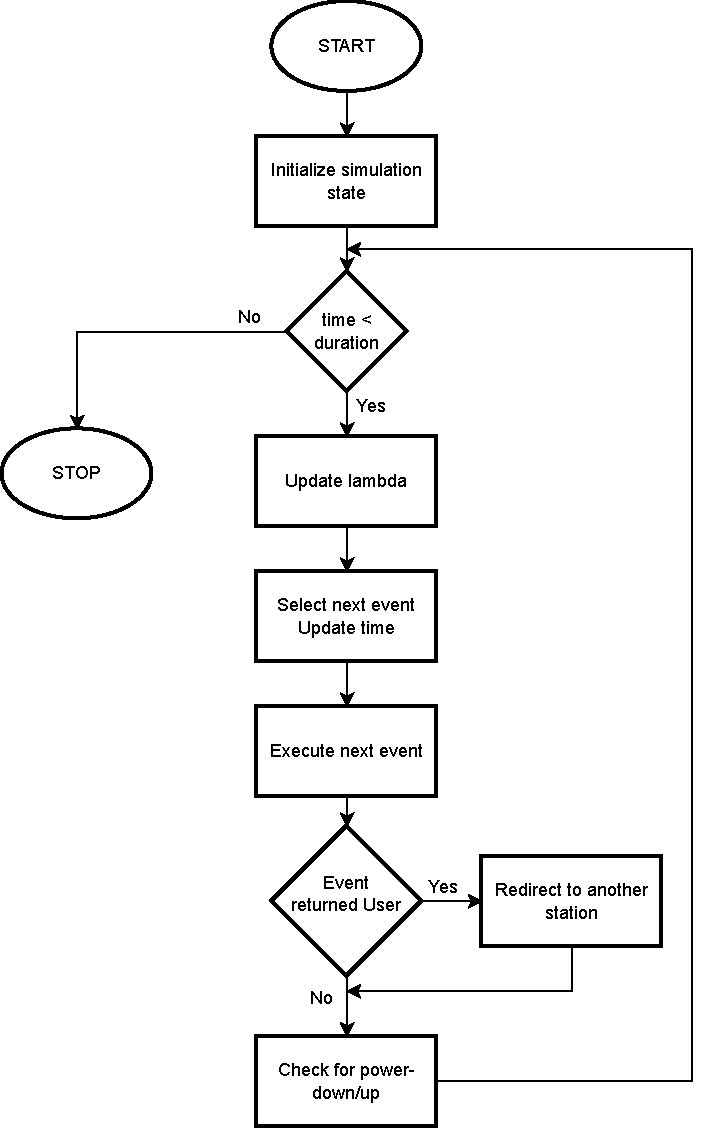
\includegraphics[scale=0.75]{img/main_loop.pdf} 
\caption{Schemat blokowy pętli głównej programu}
\label{main_loop}
\end{figure}

\begin{figure}
\center
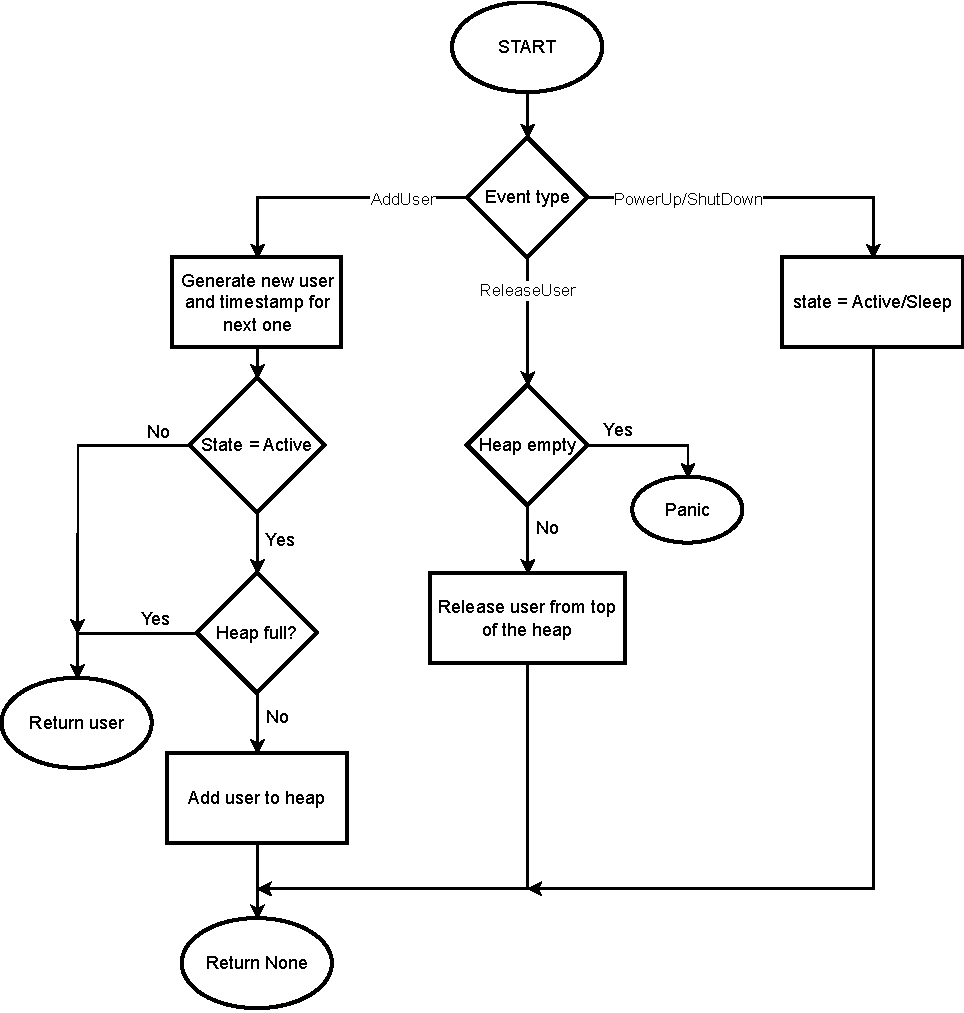
\includegraphics[scale=0.75]{img/station_event.pdf} 
\caption{Schemat blokowy pętli głównej programu}
\label{station_event}
\end{figure}


\begin{figure}
\center
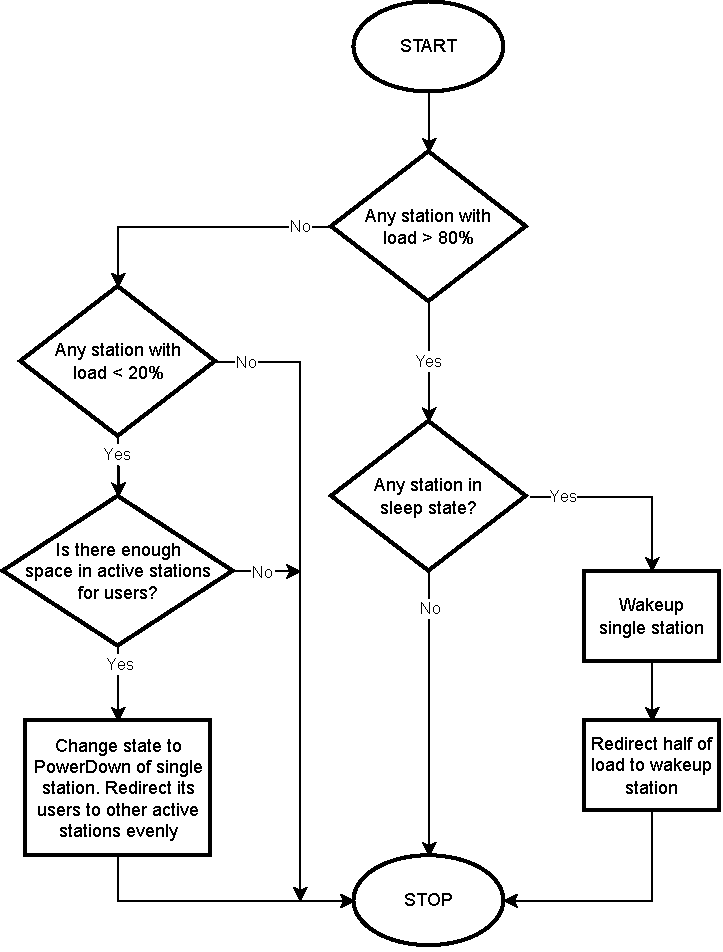
\includegraphics[scale=0.75]{img/power_up_down_logic.pdf} 
\caption{Schemat blokowy pętli głównej programu}
\label{power_up_down}
\end{figure}

\begin{figure}[h]
\center
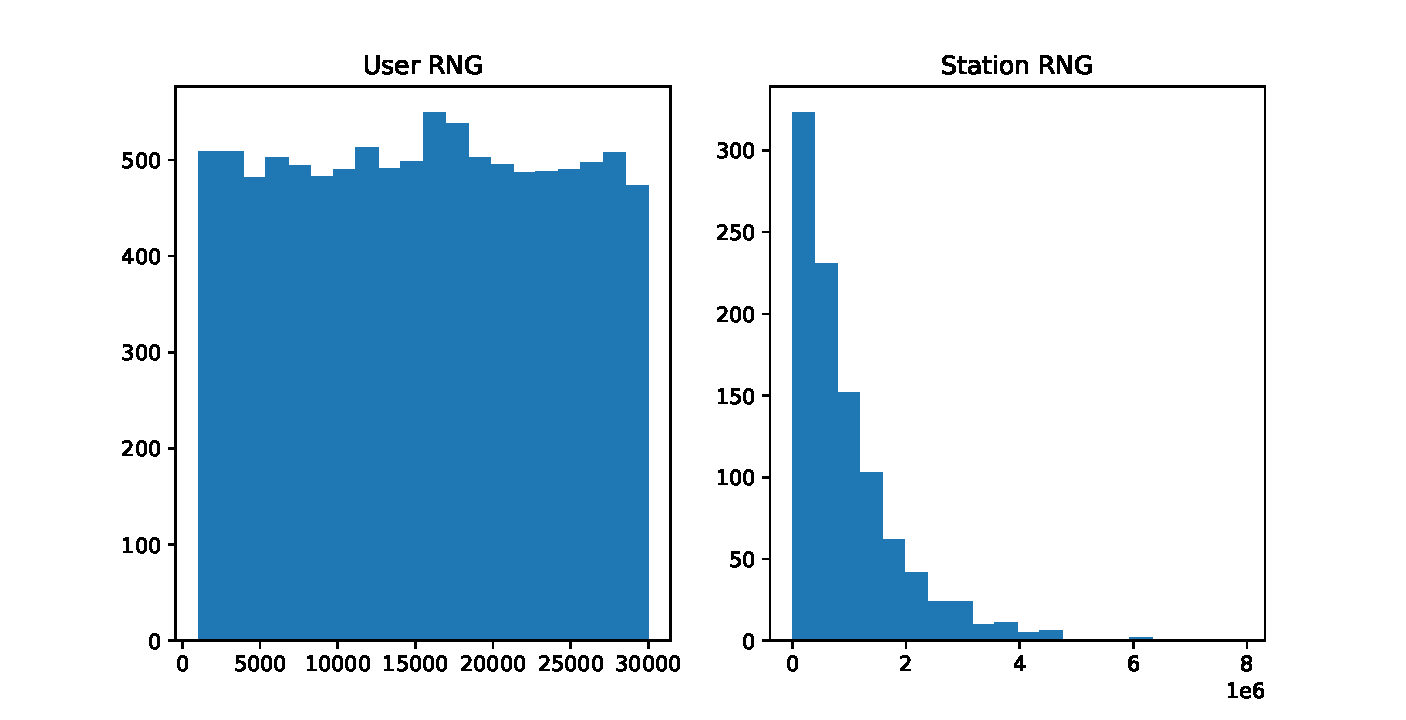
\includegraphics[scale=0.65]{img/rng.pdf} 
\caption{Histogramy reprezentujące generatory liczb losowych czasu przetwarzania użytkownika oraz czasu do pojawiania się nowego użytkownika}
\label{rng_hist}
\end{figure}
\section{Struktury}
\subsection{Struktury konfiguracyjne}
Wszystkie struktury konfiguracyjne oraz metody bezpośrednio z nimi związane znajdują się w pliku \emph{src/config.rs}
\newline\newline
\noindent Struktura \emph{Cli} zawiera pola odpowiadające wszystkim przełącznikom, których można użyć przy uruchamianiu programu. Sprawdzanie poprawności danych i konwersja na odpowiednie typy jest realizowana za pośrednictwem biblioteki \emph{Clap}.
\newline\newline
\noindent Struktura \emph{Config} zawiera wszystkie pola pliku konfiguracyjnego symulacji. Wczytywanie danych jest realizowane za pomocą bibliotek \emph{Serde} oraz \emph{toml}. Lista współczynników $\lambda$ jest reprezentowana wektorem struktur \emph{LambdaPoint}. Każda instancja zawiera dwa pola:
\begin{itemize}
\item time -- czas trwania danej fazy
\item coef -- współczynnik $\lambda$
\end{itemize}
\noindent Poprawność danych jest sprawdzana metodą \emph{validate()} zaimplementowaną dla struktury \emph{Config}.
\newline\newline
\noindent Struktura \emph{WalkOverConfig} zawiera wszystkie pola pliku konfiguracyjnego iteracji po zadanym parametrze. Wczytywanie i walidacja danych z pliku jest realizowana za pomocą bibliotek \emph{Serde} i \emph{toml}.


\subsection{Struktura użytkownika -- \emph{User}}
Struktura modelująca pojedynczego użytkownika oraz wszystkie zaimplementowane dla niej metody znajdują się w pliku \emph{src/user.rs}. Struktura zawiera unikatowy identyfikator (\emph{id}), czas pojawienia się użytkownika w systemie (\emph{start}) oraz czas zakończenia obsługi (\emph{end}), który jest sumą czasu pojawienia się i losowego czasu obsługi, losowanego z rozkładu równomiernego.
{
\fontencoding{T1}\selectfont 
\begin{minted}{rust}
pub struct User {
    pub id: usize,
    pub start: u64,
    pub end: u64,
}

impl User {
    pub fn new(id: usize, curr_time: u64, generator: &mut StdRng, cfg: &Config) -> User {
        // convert process_time from miliseconds to microseconds
        let delay: u64 =
            generator.gen_range((cfg.process_time_min * 1000)..=(cfg.process_time_max * 1000));
        User {
            id,
            start: curr_time,
            end: curr_time + delay,
        }
    }
}
\end{minted}
}

\subsection{Struktura stacji bazowej -- \emph{BaseStation}}
Struktura modelująca stację bazową i zaimplementowane na niej metody znajdują się w pliku \emph{src/basestation.rs}. Każda instancja stacji zawiera unikatowy identyfikator (\emph{id}), kopiec binarny reprezentujący bloki zasobów (\emph{resources}), znacznik czasu pojawienia się kolejnego użytkownika (\emph{next\_user\_add}), stan stacji (\emph{state}) oraz liczniki zużytej mocy (\emph{total\_power}), zużytych zasobów (\emph{total\_usage}) i czasu w trybie uśpienia (\emph{sleep\_time}). Kopiec binarny został wybrany jako głównu struktura danych w systemie ze względu na stałą złożoność $O(1)$ dostępu do najmniejszego elementu oraz logarytmiczną złożoność $O(log{n})$ dodawania i usuwania elementów z kopca.
\newline\newline
\noindent Znacznik czasu pojawienia się nowego użytkownika jest wyznaczany z rozkładu wykładniczego, którego gęstość prawdopodobieństwa określona jest wzorem:
\[ \lambda \cdot e^{-\lambda x} \]
gdzie parametr x to liczba losowa wytworzona generatorem liczb losowych.

{
\fontencoding{T1}\selectfont 
\begin{minted}{rust}
pub struct BaseStation {
    pub id: usize,
    resources: BinaryHeap<User, FnComparator<fn(&User, &User) -> Ordering>>,
    pub next_user_add: u64,
    pub state: BaseStationState,
    pub total_power: f64,
    pub total_usage: f64,
    pub sleep_time: u64,
}
\end{minted}
}

\noindent Stan stacji bazowej jest reprezentowany jednym z wariantów typu wyliczeniowego (ang. \emph{enum}) \emph{BaseStationState}. Stany \emph{PowerUp} i \emph{PowerDown}, reprezentujące stan przełączenia pomiędzy stanami aktywnym i uśpienia, przechowują znacznik czasu zakończenia tego stanu. Zdarzenia generowane przez stację są reprezentowane przez typ wyliczeniowy \emph{BaseStationEvent}.
{
\fontencoding{T1}\selectfont 
\begin{minted}{rust}
pub enum BaseStationState {
    Active,
    Sleep,
    PowerUp(u64),   // Station is during power-up process
    PowerDown(u64), // Station is during power-down process
}

pub enum BaseStationEvent {
    ReleaseUser,
    AddUser,
    PowerUp,
    ShutDown,
}
\end{minted}
}

\noindent Po zakończeniu symulacji, zawartości liczników są dzielone przez czas trwania symulacji, a następnie są zwracane jako instancja struktury \emph{BaseStationResult}.
{
\fontencoding{T1}\selectfont 
\begin{minted}{rust}
pub struct BaseStationResult {
    pub average_power: f64,
    pub average_usage: f64,
    pub average_sleep_time: f64,
}
\end{minted}
}

\subsection{Struktura kontenera symulacji -- \emph{SimContainer}}
Struktura \emph{SimContainer}, zdefiniowana w pliku \emph{src/sim\_container.rs}, jest abstrakcyjną strukturą modelującą system. Zawiera jedynie instancje struktur konfiguracyjnych. Stan symulacji, modelowany strukturą \emph{SimState}, jest tworzony osobno dla każdego przebiegu symulacji. Niezależność przebiegów umożliwia proste zrównoleglenie obliczeń za pomocą biblioteki \emph{Rayon}. Dwie najważniejsze metody zaimplementowane na strukturze \emph{SimContainer} to:
\begin{itemize}
\item \emph{simulate()} -- tworzy nową instancję stanu i uruchamia jeden przebieg symulacji. Wyniki są zwracane jako instancja struktury \emph{SimResults}, które jest zdefiniowana w pliku \emph{src/sim\_container/sim\_results.rs},
\item \emph{run()} -- wywołuje równolegle metodę \emph{simulate()} a następnie uśrednia uzyskane wyniki, które są zwracane jako pojedyncza instancja struktury \emph{SimResults}, która zawiera uśrednione wyniki z całego systemu oraz wektor wyników z poszczególnych stacji
\end{itemize}
{
\fontencoding{T1}\selectfont 
\begin{minted}{rust}
pub struct SimContainer {
    cli: Cli,
    cfg: Config,
}

pub struct SimState {
    pub time: u64,
    pub next_user_id: usize,
    pub lambda: f64,
    pub lambda_update_time: u64,
    pub lambda_update_idx: usize,
    pub all_users: usize,
    pub redirected_users: usize,
    pub dropped_users: usize,
}

pub struct SimResults {
    pub average_usage: f64,
    pub average_power: f64,
    pub average_drop_rate: f64,
    pub total_users: usize,
    pub dropped_users: usize,
    pub stations: Vec<BaseStationResult>,
}
\end{minted}
}

\newpage
\section{Generatory liczb losowych}
Na początku każdego przebiegu symulacji tworzona jest instancja generatora liczb losowych \emph{StdRng}.
Ziarno każdego generatora jest losowane ze źródeł zapewnionych przez dany system operacyjny na podstawie jego entropii. Histogramy generowanych liczb losowych z rozkładu równomiernego i wykładniczego przedstawiono na rysunku \ref{rng_hist}.
Ponieważ każda iteracja symulacji musi posiadać niezależny stan wewnętrzny, aby umożliwić wykonywanie równoległe przebiegów, każda iteracja posiada osobny generator liczb losowych z indywidualnie wygenerowanym ziarnem. To rozwiązanie umożliwia także wyznaczanie parametrów statystycznych na podstawie uzyskanych wyników z wielu, krótkich przebiegów, metodą niezależnych replikacji (ang. \emph{independent replication method}). Wymaga ona aby faza początkowa, w której system przechodzi do stanu ustalonego, była krótka względem całkowitego czasu eksperymentu. Tą własność potwierdzono eksperymentem opisanym w sekcji \ref{initial_phase_section}.

\begin{figure}[h]
\center
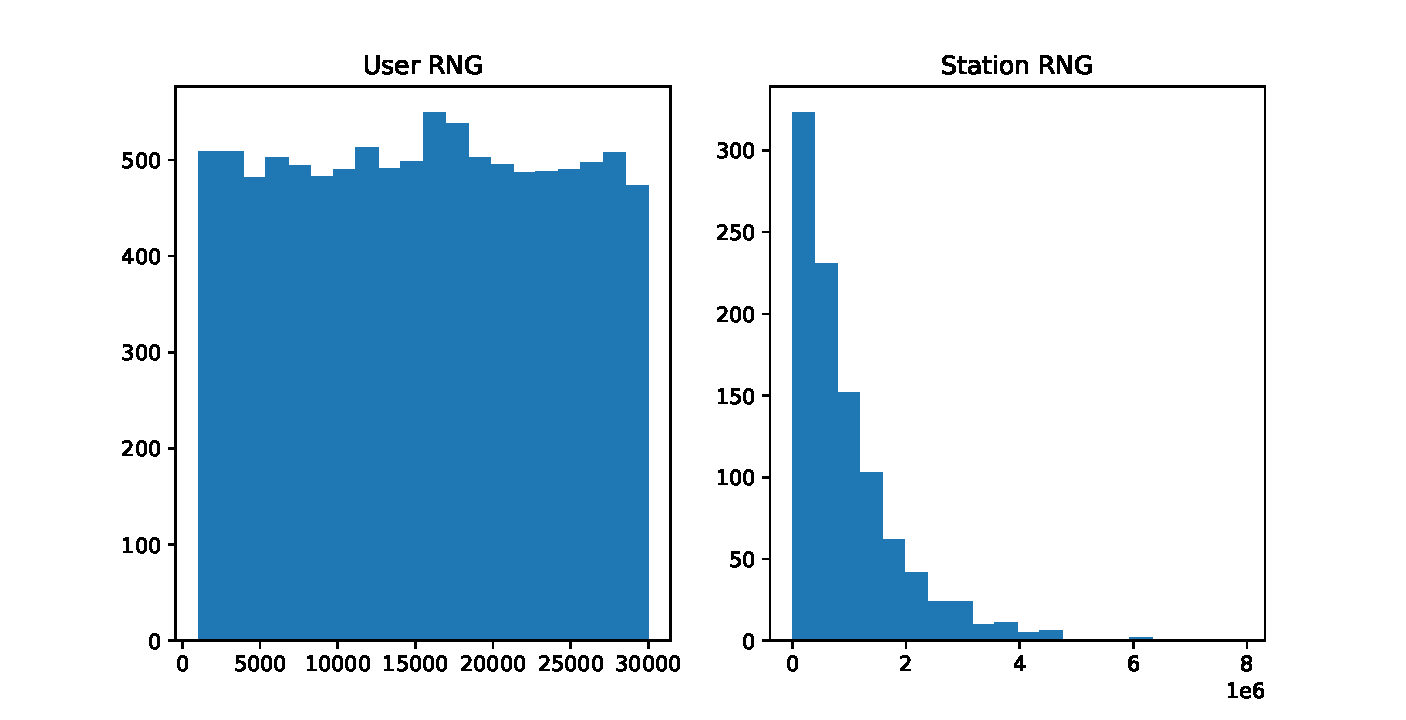
\includegraphics[scale=0.65]{img/rng.pdf} 
\caption{Histogramy reprezentujące generatory liczb losowych czasu przetwarzania użytkownika (\emph{User RNG}) oraz czasu do pojawiania się nowego użytkownika (\emph{Station RNG})}
\label{rng_hist}
\end{figure}
\newpage
\section{Testowanie programu}
Poszczególne funkcjonalności programu zostały przetestowane za pomocą testów jednostkowych (ang. \emph{unit test}). Testy dotyczące danych funkcji są zawarte w module \emph{mod test}, w tym samym pliku źródłowym oraz bazują na wbudowanej infrastrukturze testowej ekosystemu języka \emph{Rust}. Aby uruchomić wszystkie testy wystarczy użyć komendy \emph{cargo test} w głównym folderze projektu. Zrzut ekranu, przedstawiający pozytywny wynik wszystkich testów, zawarto na rysunku \ref{regression}.

\begin{figure}[h]
\center
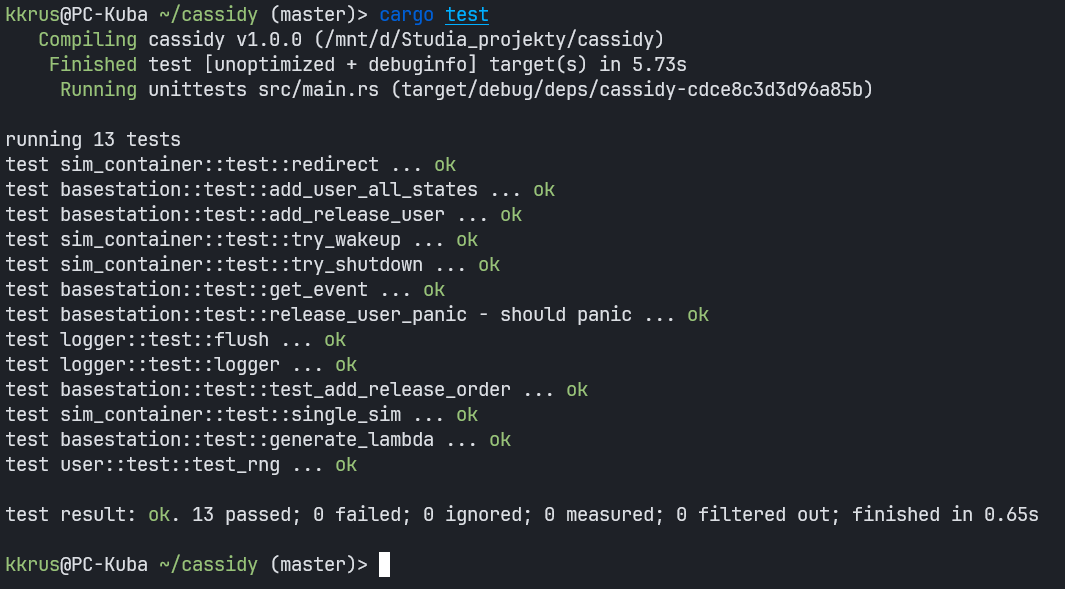
\includegraphics[scale=0.55]{img/tests.png} 
\caption{Przykładowy wynik komendy \emph{cargo test}}
\label{regression}
\end{figure}

\noindent W procesie testowania aplikacji wykorzystywano także generowane pliki \emph{log} oraz wymienione w sekcji \ref{python_scripts} skrypty napisane w języku \emph{Python}. Umożliwiają one ręczne oraz automatyczne sprawdzanie poprawności działania pętli głównej programu. Fragment przykładowego pliku \emph{event log} przedstawiono poniżej. Pierwsza kolumna zawiera znacznik czasu wyrażony w mikrosekundach. Następnie podany jest rodzaj zdarzenia oraz dotyczące go informacje.

\begin{verbatim}
10009189   UserAdd       Station id: 2   User id: 14, end time: 12492641 next user: 11003934
10941299   UserRelease   Station id: 0   User id: 3, end time: 10941299
11003934   UserAdd       Station id: 2   User id: 15, end time: 17544415 next user: 17034435
11161844   UserRelease   Station id: 0   User id: 5, end time: 11161844
12097745   UserAdd       Station id: 0   User id: 16, end time: 36047089 next user: 13170839
12492641   UserRelease   Station id: 2   User id: 14, end time: 12492641
13100375   UserRelease   Station id: 2   User id: 1, end time: 13100375
13170839   UserAdd       Station id: 0   User id: 17, end time: 34192635 next user: 14459706
14299594   UserRelease   Station id: 0   User id: 8, end time: 14299594
\end{verbatim}


\newpage
\section{Wyniki symulacji} \label{initial_phase_section}
\subsection{Wyznaczenie długości fazy początkowej}
Długość fazy początkowej wyznaczono za pomocą binarnego pliku \emph{log} zawierającego ilość zajętych bloków zasobów każdej stacji w funkcji czasu. Uzyskane wyniki dla pięciu różnych wartości parametru $\lambda$ przedstawiono w tabeli \ref{initial_phase_table}. Na podstawie uzyskanych wyników stwierdzono skracanie czasu trwania fazy początkowej wraz ze wzrostem wartości parametru $\lambda$ oraz uznano jej wpływ na wyniki trwania eksperymentu za nieznaczące. Przykładowy wykres, na podstawie którego wyznaczono wyniki przedstawiono na rysunku \ref{initial_phase_lambda_20}. Analizując wyniki należy mieć na uwadze subiektywność uzyskanych wyników, ze względu na nieprecyzyjną definicję końca fazy początkowej.

\begin{table}[h]
\caption{Wyznaczony czas fazy początkowe dla różnych wartości $\lambda$}
\label{initial_phase_table}
\begin{center}
\renewcommand{\arraystretch}{1.5}
\begin{tabular}{|l|l|l|l|l|l|}
\hline 
Lambda & 20 & 25 & 30 & 35 & 40 \\ 
\hline 
Czas fazy początkowej [s] & 38 & 36 & 30 & 27 & 20 \\ 
\hline
\end{tabular}
\end{center}
\end{table}

\begin{figure}[h]
\center
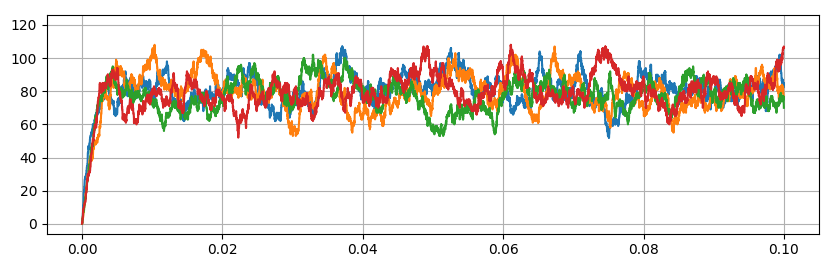
\includegraphics[scale=0.65]{img/initial_phase_lambda_20.png} 
\caption{Wykres ilości zajętych bloków zasobów stacji bazowych w funkcji czasu wyrażonego w godzinach. Parametr $\lambda$ podczas symulacji był równy 20}
\label{initial_phase_lambda_20}
\end{figure}

\subsection{Wyznaczenie granicznej wartości $\lambda$, dla której nie stracono żadnego użytkownika}
Aby wyznaczyć wartość graniczną, uruchomiono symulację dla wartości $\lambda$ z zakresu $<10; 50>$ użytkowników na sekundę, z krokiem 5. Każda próbka została uśredniona z 10 iteracji. W trakcie symulacji logika odpowiadająca za usypianie stacji była wyłączona. Wyniki symulacji, wraz z obliczonymi przedziałami ufności, przedstawiono w tabeli \ref{dropped_users_by_lambda_table} oraz na rysunku \ref{dropped_users_lambda}. Ostatnią wyznaczoną wartością $\lambda$, dla której nie stracono żadnego użytkownika, to 30 użytkowników na sekundę.

\begin{table}[]
\centering
\renewcommand{\arraystretch}{1.5}
\caption{Wyniki pomiaru ilości traconych użytkowników w systemie w funkcji wartości parametru $\lambda$}
\label{dropped_users_by_lambda_table}
\begin{tabular}{|l|l|l|}
\hline
lambda & \begin{tabular}[c]{@{}l@{}}Ilość straconych\\ użytkowników\end{tabular} & Przedział ufności \\ \hline
10 & 0 & 0 \\ \hline
15 & 0 & 0 \\ \hline
20 & 0 & 0 \\ \hline
25 & 0 & 0 \\ \hline
30 & 0 & 0 \\ \hline
35 & 168720 & 1152 \\ \hline
40 & 856671 & 1686 \\ \hline
45 & 1700934 & 1755 \\ \hline
50 & 3799727 & 1605 \\ \hline
\end{tabular}
\end{table}

\begin{figure}[h!]
\center
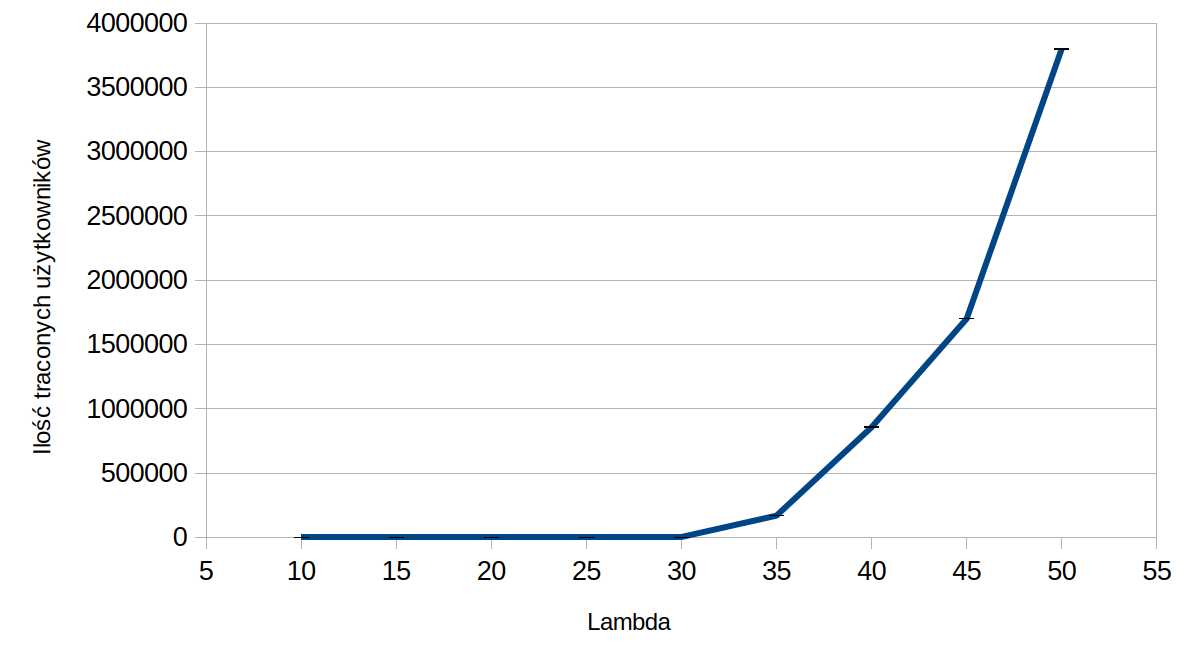
\includegraphics[scale=0.45]{img/dropped_users_by_lambda.png} 
\caption{Wykres liczby traconych użytkowników w funkcji wartości parametru $\lambda$}
\label{dropped_users_lambda}
\end{figure}

\newpage
\subsection{Wyznaczenie granicznej wartości progu L, dla której straty użytkowników są poniżej 5\%}\label{drop_rate_5_section}
Aby wyznaczyć wartość graniczną, uruchomiono symulację dla wartości progu L z zakresu $<5; 40>\%$, z krokiem 5. Każda próbka została uśredniona z 10 iteracji. W trakcie symulacji parametr $\lambda$ wynosił 35. Wynik symulacji przedstawiono na rysunku \ref{dropped_users_iter_l}. Z wyników symulacji wynika, że ilość traconych użytkowników w systemie nie zależy od wartości progu L. Eksperyment powtórzono dla wartości $\lambda = $ 40 oraz 50, których wyniki przedstawiono na rysunkach \ref{dropped_users_iter_l2} i \ref{dropped_users_iter_l3}.
W każdym przypadku różnice pomiędzy uzyskanymi wynikami są pomijalnie małe. Wynika to najprawdopodobniej z zastosowanego algorytmu usypiania i wybudzania stacji bazowych, który został zaprojektowany tak aby maksymalnie zminimalizować ilość traconych użytkowników w systemie. Analizując wykres zużycia zasobów stacji w czasie, przedstawionego na rysunku \ref{usage_over_time}, można zauważyć, że badana wartość utrzymuje się na w przybliżeniu stałym poziomie zależnym od współczynnika $\lambda$ w danej fazie. Aby wygenerować straty użytkowników przekraczające 5\%, parametr $\lambda$ powinien być duży, na przykład z zakresu $<50;70>$ użytkowników na sekundę, aby zapełnić bloki zasobów we wszystkich stacjach.
Zakres ten został wyznaczony osobnymi symulacjami, z wyłączoną logiką odpowiadająca za usypianie i wybudzanie stacji. Duża wartość parametru $\lambda$ jest także wymagana aby w systemie pojawiła się wystarczająca liczba użytkowników, aby przepełnić aktywne stacje, zanim zostanie wybudzona stacja uśpiona. Natomiast aby próg L, wskazujący poniżej jakiej wartości stacja bazowa może przejść w stan uśpienia, miał wpływ na przebieg symulacji, wartość parametru $\lambda$ musi być niska, aby zużycie bloków zasobów stacji spadło poniżej progu L. Jest to sprzeczne z postawionymi wcześniej założeniami i dlatego taka sytuacja nie zachodzi w systemie, dla podanych w treści zadania parametrów. Dlatego do dalszej części tego zadania, opisanego w sekcji \ref{get_params_section} przyjęto następujące parametry symulacji:
\begin{itemize}
\item Lambda = 43 użytkowników na sekundę
\item L = 20\%
\end{itemize}

\begin{figure}[h!]
\center
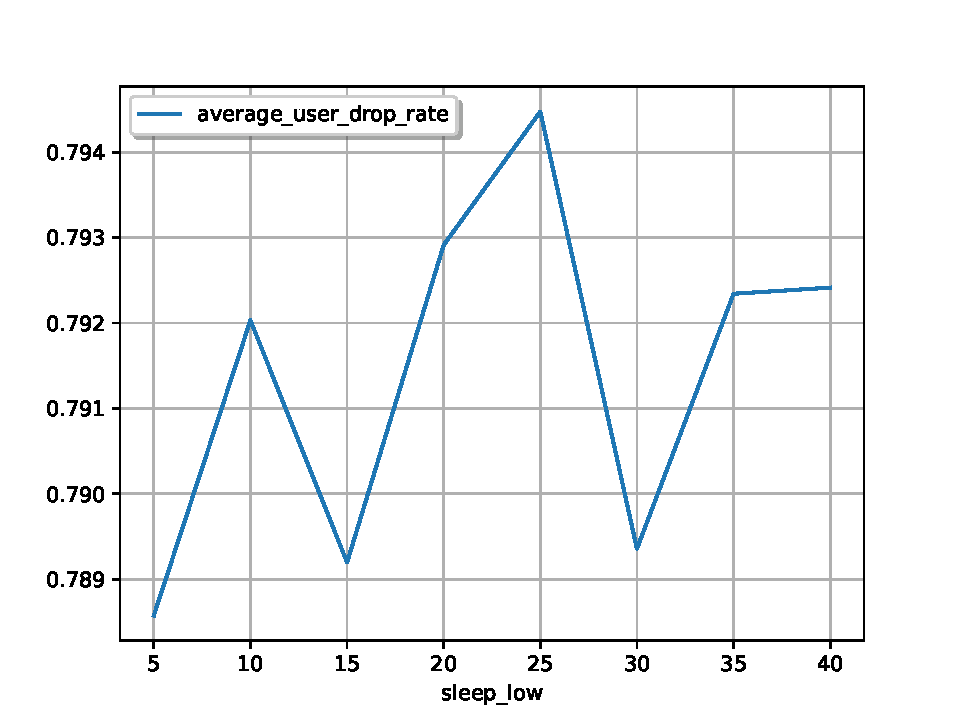
\includegraphics[scale=0.65]{img/drop_rate_lambda_35.pdf} 
\caption{Wykres procentu traconych użytkowników w funkcji wartości parametru L. W trakcie symulacji parametr $\lambda$ wynosił 35.}
\label{dropped_users_iter_l}
\end{figure}

\begin{figure}[h!]
\center
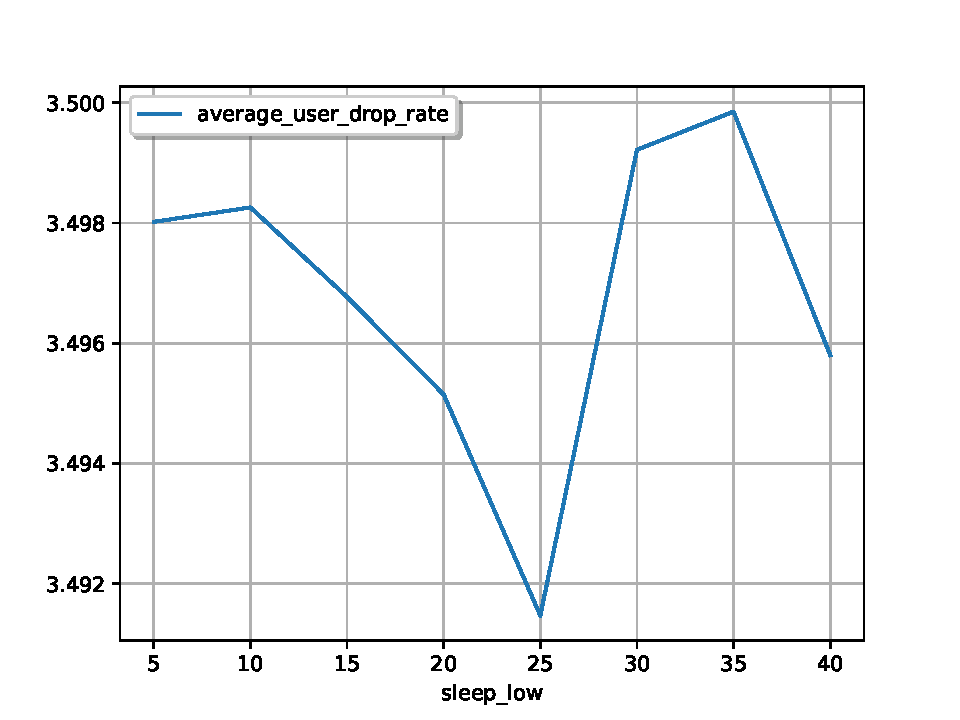
\includegraphics[scale=0.65]{img/drop_rate_lambda_40.pdf} 
\caption{Wykres procentu traconych użytkowników w funkcji wartości parametru L. W trakcie symulacji parametr $\lambda$ wynosił 40.}
\label{dropped_users_iter_l2}
\end{figure}

\begin{figure}[h!]
\center
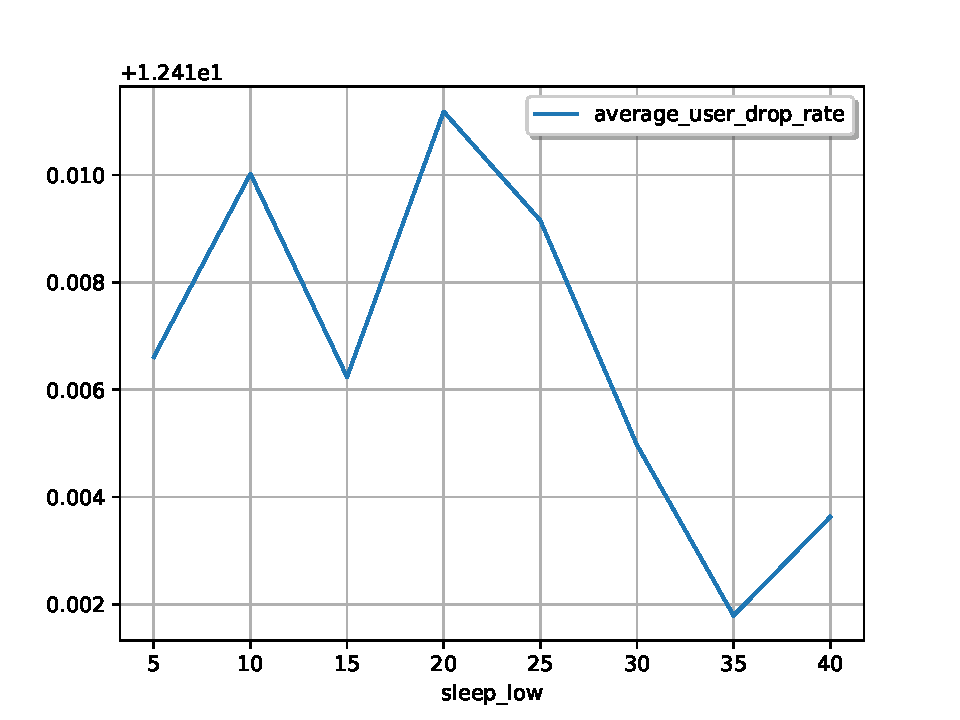
\includegraphics[scale=0.65]{img/drop_rate_lambda_50.pdf} 
\caption{Wykres procentu traconych użytkowników w funkcji wartości parametru L. W trakcie symulacji parametr $\lambda$ wynosił 50.}
\label{dropped_users_iter_l3}
\end{figure}

\begin{figure}[h!]
\center
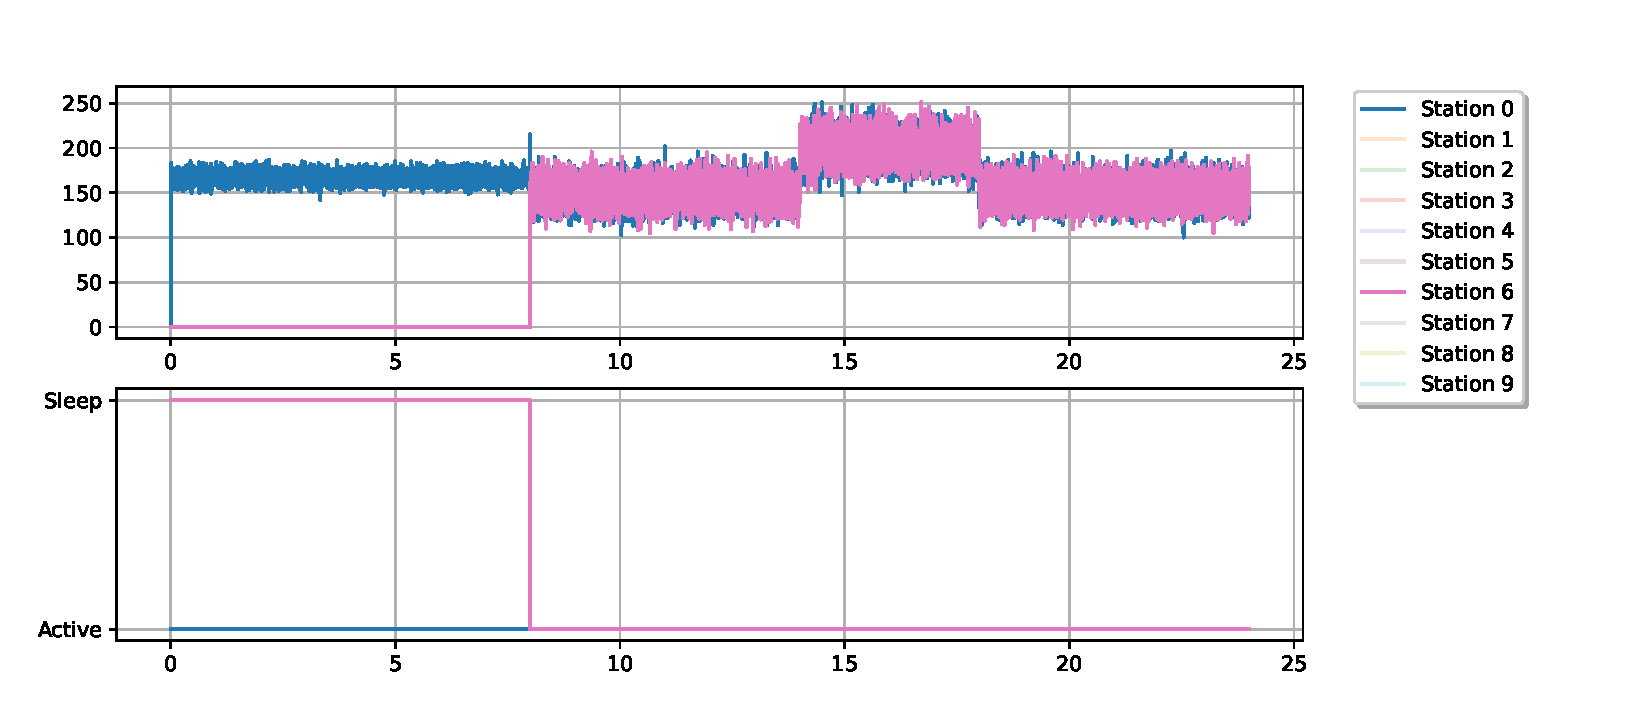
\includegraphics[scale=0.65]{img/usage_over_time.pdf} 
\caption{Wykres zużycia zasobów stacji bazowych nr 0 i 6 w funkcji czasu symulacji}
\label{usage_over_time}
\end{figure}

\newpage\newpage
\subsection{Wyznaczenie uśrednionych parametrów systemu} \label{get_params_section}
Uśrednione parametry systemu wyznaczono symulacją uśrednioną z 20 iteracji, gdzie parametr $\lambda$ wynosił 43 a próg L był równy 20\%. Wyniki symulacji oraz raport końcowy z programu przedstawiono odpowiednio w tabeli \ref{params_table} oraz na rysunku \ref{sim_results_average}. Ponieważ ilość użytkowników napływających do systemu była większa od pojemności stacji bazowych, wszystkie uśpione stacje zostały wybudzone w początkowej fazie symulacji, stąd średnia moc pobierana przez stacje wynosi 200W a średni czas uśpienia to 0\%. Parametry statystyczne zostały wyznaczone na podstawie wyników pośrednich, uzyskanych z użyciem przełącznika \emph{-{}-show-partial-results}, za pomocą wbudowanych funkcji programu \emph{Excel}.
\newline\newline
\begin{table}[]
\renewcommand{\arraystretch}{1.5}
\centering
\caption{Wyniki mierzonych parametrów systemu w każdej iteracji}
\label{params_table}
\begin{tabular}{|p{0.2\textwidth}|p{0.15\textwidth}|p{0.15\textwidth}|p{0.15\textwidth}|p{0.15\textwidth}|}
\hline
Iteracja & Średnie zużycie zasobów [\%] & Średni pobór mocy [W] & Średni procent traconych użytkowników & Średni czas uśpienia \\ \hline
0 & 84,891 & 200 & 4,899 & 0 \\ \hline
1 & 84,877 & 200 & 4,897 & 0 \\ \hline
2 & 84,899 & 200 & 4,902 & 0 \\ \hline
3 & 84,897 & 200 & 4,894 & 0 \\ \hline
4 & 84,863 & 200 & 4,890 & 0 \\ \hline
5 & 84,897 & 200 & 4,896 & 0 \\ \hline
6 & 84,863 & 200 & 4,905 & 0 \\ \hline
7 & 84,864 & 200 & 4,876 & 0 \\ \hline
8 & 84,890 & 200 & 4,909 & 0 \\ \hline
9 & 84,884 & 200 & 4,891 & 0 \\ \hline
10 & 84,898 & 200 & 4,890 & 0 \\ \hline
11 & 84,890 & 200 & 4,868 & 0 \\ \hline
12 & 84,873 & 200 & 4,896 & 0 \\ \hline
13 & 84,892 & 200 & 4,892 & 0 \\ \hline
14 & 84,896 & 200 & 4,880 & 0 \\ \hline
15 & 84,874 & 200 & 4,896 & 0 \\ \hline
16 & 84,893 & 200 & 4,895 & 0 \\ \hline
17 & 84,880 & 200 & 4,906 & 0 \\ \hline
18 & 84,901 & 200 & 4,896 & 0 \\ \hline
19 & 84,891 & 200 & 4,891 & 0 \\ \hline
Wartość średnia & 84,886 & 200 & 4,893 & 0 \\ \hline
Odchylenie standardowe & 0,0126 & 0 & 0,010 & 0 \\ \hline
Przedział ufności & 0,006 & - & 0,004 & - \\ \hline
\end{tabular}
\end{table}

\begin{figure}[h!]
\center
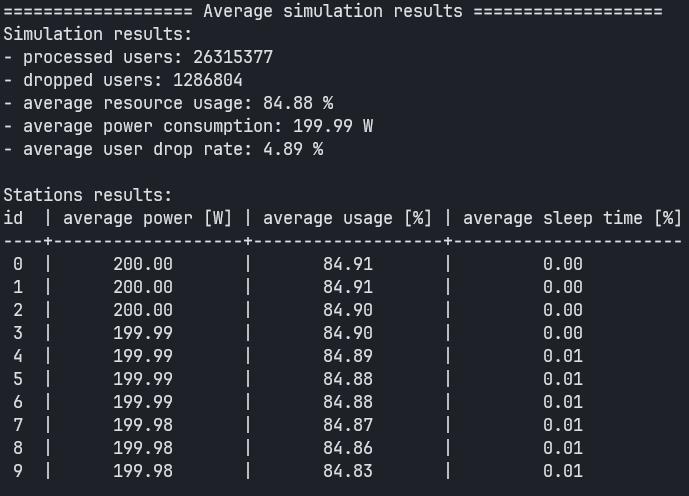
\includegraphics[scale=0.6]{img/sim_results_sleep_lambda_43.png} 
\caption{Raport wynikowy symulacji dla parametrów $\lambda$ = 43 oraz L = 20, uśredniony z 20 iteracji}
\label{sim_results_average}
\end{figure}

\newpage
\subsection{Wyznaczenie średniego zużycia energii w funkcji progu L} \label{power_l_plot}
Symulację wykonano dla wartości progu L z zakresu $<5:40>$ z krokiem równym 5, dla wartości parametru $\lambda$ = 20. Wyniki symulacji przedstawiono w tabeli \ref{power_usage_by_l} oraz na rysunku \ref{power_usage_lambda_sleep}. Każda próbka wykresu została uśredniona z 10 iteracji. Z analizy uzyskanego wykresu wynika że wraz ze wzrostem progu uśpienia L, dla niskich wartości $\lambda$, średni pobór mocy przez stacje bazowe maleje. Na rysunku \ref{usage_over_time_sleep} przedstawiono wykres zużycia zasobów stacji 0 i 7 w funkcji czasu. Stacja numer 7 została aktywowany po rozpoczęciu fazy największego ruchu (gdy współczynnik $\lambda\_coef$ = 1) oraz została wyłączona gdy generowany ruch zmalał. Dzięki temu średni pobór mocy w systemie zmalał, względem symulacji gdy próg uśpienia miał niższą wartość lub gdy logika odpowiedzialna za usypianie stacji była wyłączona.

\begin{table}[h]
\renewcommand{\arraystretch}{1.5}
\centering
\caption{Wyniki pomiaru średniego zużycia mocy w funkcji wartości parametru L}
\label{power_usage_by_l}
\begin{tabular}{|l|l|l|}
\hline
Próg L {[}\%{]} & Średnie zużycie mocy {[}W{]} & Przedział ufności \\ \hline
5 & 154,633 & 2,060 \\ \hline
10 & 153,566 & 1,833 \\ \hline
15 & 155,074 & 2,759 \\ \hline
20 & 155,949 & 3,213 \\ \hline
25 & 153,625 & 2,151 \\ \hline
30 & 149,099 & 1,698 \\ \hline
35 & 146,011 & 2,196 \\ \hline
40 & 139,263 & 0,989 \\ \hline
\end{tabular}
\end{table}

\begin{figure}[h!]
\center
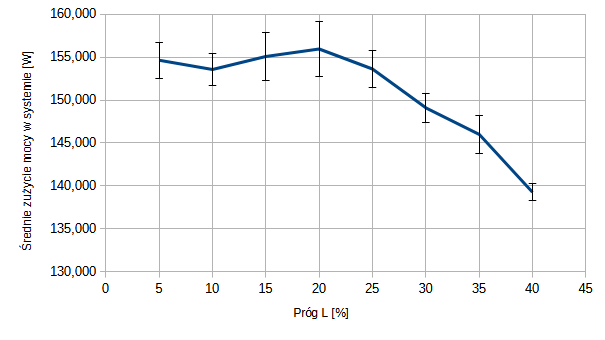
\includegraphics[scale=0.75]{img/power_by_l.png} 
\caption{Wykres średniego poboru mocy przez stacje bazowe w funkcji wartości progu L. W trakcie symulacji parametr $\lambda$ był równy 20}
\label{power_usage_lambda_sleep}
\end{figure}

\begin{figure}[h]
\center
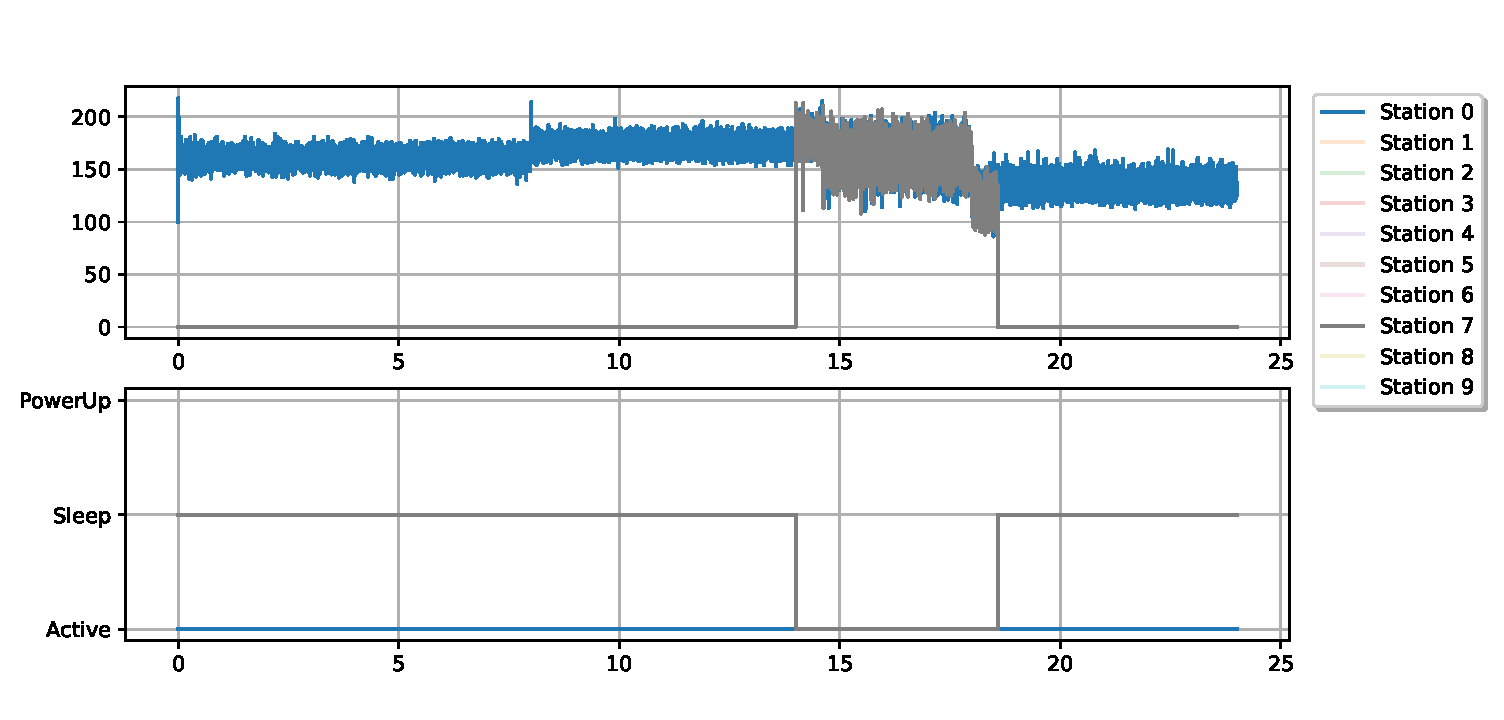
\includegraphics[scale=0.65]{img/usage_over_time_sleep.pdf} 
\caption{Wykres średniego poboru mocy przez stacje bazowe w funkcji wartości progu L}
\label{usage_over_time_sleep}
\end{figure}

\subsection{Wyznaczenie średniej ilości traconych użytkowników w funkcji progu L} \label{drop_l_plot}
Z przyczyn wymienionych w sekcji \ref{drop_rate_5_section}, liczba traconych użytkowników nie zależy od wartości progu L oraz, ponieważ w trakcie symulacji parametr $\lambda$ był równy 20, jest równa zero.

\begin{figure}[h!]
\center
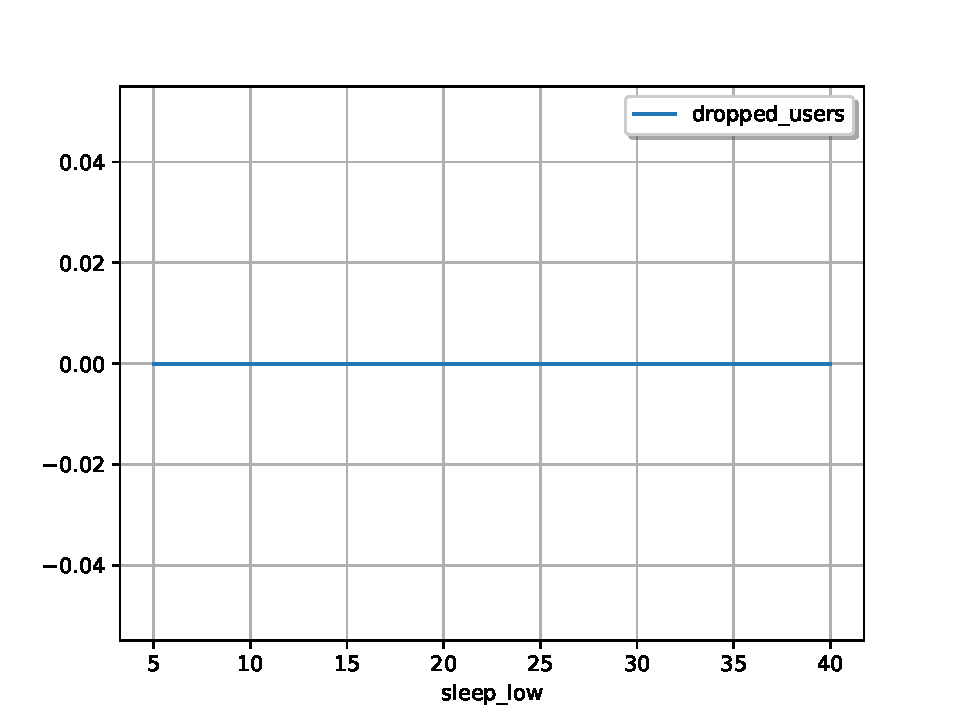
\includegraphics[scale=0.65]{img/dropped_users_lambda_20.pdf} 
\caption{Wykres średniego ilości traconych użytkowników w funkcji wartości progu L}
\label{drop_over_time_sleep}
\end{figure}


\end{document}